\subsection{Configuration B: CPU Laptop Model}
\label{sec:cpu}
Configuration~B repeats the experiment on the laptop CPU with SmolLM2-360M as target (8.68M LoRA parameters, 2 epochs, \TTrainHours{}\,h of training) and SmolLM2-135M as draft. It matters for two reasons: it is the model the locally hosted application loads by default, and it shows how much of Configuration~A's behaviour depends on model scale.

\textbf{Fine-tuning and before/after.} Table~\ref{tab:epochsB} and Fig.~\ref{fig:trainB} show that after epoch~1 the model's validation accuracy (0.621) and macro-F1 (0.215) are \emph{identical} to the majority-label baseline: it had learned the answer format and the common label, nothing more. After epoch~2 (selected, validation macro-F1 0.317) it has started to discriminate inclusion classes. Table~\ref{tab:mainB} gives the before/after comparison on identical rows. The zero-shot 360M base model reaches test accuracy \BaseAcc{} and macro-F1 \BaseMF{} (it follows the schema, 0 invalid outputs, but cites no evidence at all: evidence F1 0.000); after fine-tuning, accuracy is \TestAcc{} (interval \TestAccLo--\TestAccHi), macro-F1 \TestMF{} (interval \TestMFLo--\TestMFHi) and micro evidence F1 \TestEvF{} (interval \TestEvFLo--\TestEvFHi). \textbf{This is the same accuracy as the majority baseline} (\MajAcc{}), and the macro-F1 interval contains the baseline's \MajMF{}; with 8 test patients we therefore cannot claim a reliable improvement over trivial prediction for this configuration, only a point-estimate gain in macro-F1 (0.333 vs.\ 0.272) driven by inclusion criteria. Validation shows the same picture (0.684 accuracy and 0.317 macro-F1 against 0.621 and 0.215 for the majority label).

\textbf{Per-class behaviour.} For exclusion criteria the fine-tuned model answers \emph{not excluded} on all 131 rows, i.e.\ it reproduces the majority label exactly (exclusion accuracy 0.695, macro-F1 0.273), and for inclusion criteria it answers \emph{not enough information} 57 times and \emph{included} 18 times (Table~\ref{tab:pcBcpu}, Fig.~\ref{fig:cmB}): \emph{included} reaches only P~0.44, R~0.30, F1~0.36 against 0.79, 0.70 and 0.75 for the 1.7B model, and \emph{not included} and \emph{not applicable} are never predicted. \emph{Not enough information} for inclusion criteria is its best class (F1 0.63).

\textbf{Evidence.} Micro precision is 0.350 but recall only 0.074 (inclusion: P~0.350, R~0.113, F1~0.171; exclusion: nothing cited); on evidence-bearing records the macro F1 is 0.109, whereas the all-record macro F1 of 0.707 merely reflects that the model leaves \EmptyOK{} of the empty-gold records empty (\EmptyFalseCit{} spurious citations).

\textbf{Errors.} Of \NTest{} test rows 101 are correct in label and evidence, 50 are false decisions (gold \emph{not enough information} 36 or \emph{not applicable} 14, answered \emph{not excluded} 40 times and \emph{included} 10 times), 28 have the right label with different evidence, 26 are missed decisions (a decisive gold label answered \emph{not enough information} or \emph{not applicable}) and 1 is a \emph{not applicable} confusion (Table~\ref{tab:errcatB}); 131 predictions carry a decisive label without any cited sentence, 115 of which also have empty expert evidence and 16 of which do not. The twelve-case listing for Configuration~A (Table~\ref{tab:errA}) illustrates the same failure types; the CPU cases are in \texttt{results/error\_analysis\_cpu\_finetuned\_test.md}. The comparison with Configuration~A suggests that, on this data, a 1.7B model with three epochs begins to learn inclusion reasoning (included recall 0.70 vs.\ 0.30, evidence micro-F1 0.384 vs.\ 0.123) whereas a 360M model with two epochs mostly learns the label prior; both collapse on exclusion criteria.

\begin{table}[t]\centering\caption{Config.~B target (SmolLM2-360M + LoRA, CPU): validation after each epoch ($^*$ = selected).}\label{tab:epochsB}
\small\begin{tabular}{rrrrr}\toprule
Epoch & Val. loss & Val. acc. & Val. macro-F1 & Val. evid. F1 \\\midrule
1 & 0.207 & 0.621 & 0.215 & 0.214 \\
2$^*$ & 0.189 & 0.684 & 0.317 & 0.196 \\
\bottomrule\end{tabular}
\end{table}
\begin{figure}[t]\centering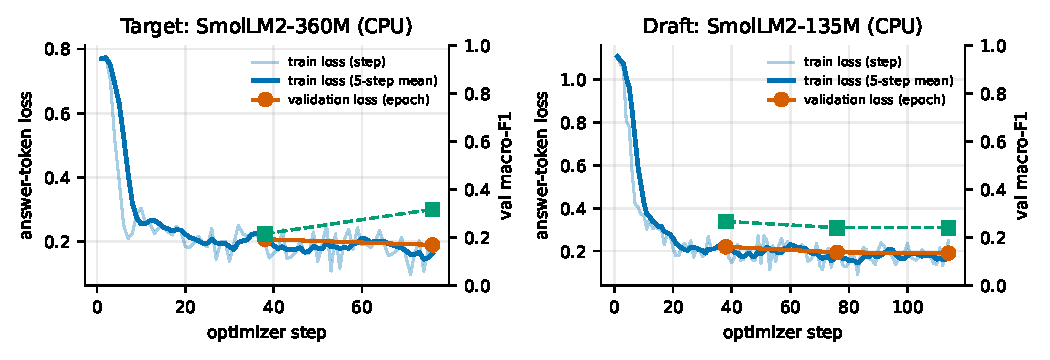
\includegraphics[width=\columnwidth]{fig_training.pdf}
\caption{Config.~B training curves (CPU): target 360M and draft 135M.}\label{fig:trainB}\end{figure}
\begin{table*}[t]\centering\caption{Config.~B (CPU): majority baseline, base zero-shot and fine-tuned SmolLM2-360M on the same rows.}\label{tab:mainB}
\small\begin{tabular}{llrrrrrrr}\toprule
Split & Model & Acc. & mF1 & Incl. acc. & Incl. mF1 & Excl. acc. & Excl. mF1 & Invalid \\\midrule
Val. & majority label & 0.621 & 0.215 & 0.409 & 0.145 & 0.721 & 0.210 & 0 \\
& base zero-shot & 0.495 & 0.229 & 0.136 & 0.113 & 0.664 & 0.276 & 0 \\
& fine-tuned & 0.684 & 0.317 & 0.606 & 0.310 & 0.721 & 0.210 & 0 \\
\midrule
Test & majority label & 0.626 & 0.272 & 0.507 & 0.168 & 0.695 & 0.273 & 0 \\
& base zero-shot & 0.437 & 0.234 & 0.120 & 0.070 & 0.618 & 0.350 & 0 \\
& fine-tuned & 0.626 & 0.333 & 0.507 & 0.247 & 0.695 & 0.273 & 0 \\
\bottomrule\end{tabular}
\end{table*}
\begin{table}[t]\centering\caption{Config.~B fine-tuned model, test split: per-class P, R, F1 and support.}\label{tab:pcBcpu}
\footnotesize\begin{tabular}{llrrrr}\toprule
Scope & Class & P & R & F1 & Support \\\midrule
inclusion & included & 0.444 & 0.296 & 0.356 & 27 \\
 & not included & 0.000 & 0.000 & 0.000 & 7 \\
 & not enough info. & 0.526 & 0.789 & 0.632 & 38 \\
 & not applicable & 0.000 & 0.000 & 0.000 & 3 \\
\midrule
exclusion & excluded & 0.000 & 0.000 & 0.000 & 0 \\
 & not excluded & 0.695 & 1.000 & 0.820 & 91 \\
 & not enough info. & 0.000 & 0.000 & 0.000 & 28 \\
 & not applicable & 0.000 & 0.000 & 0.000 & 12 \\
\bottomrule\end{tabular}
\end{table}
\begin{figure*}[t]\centering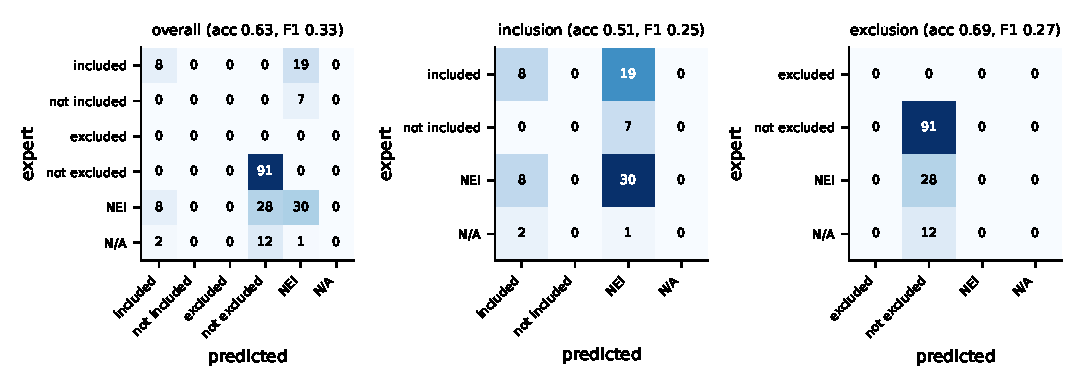
\includegraphics[width=.85\textwidth]{fig_confusion.pdf}
\caption{Config.~B confusion matrices on the test split.}\label{fig:cmB}\end{figure*}
\begin{table}[t]\centering\caption{Config.~B test errors by category.}\label{tab:errcatB}
\small\begin{tabular}{lr}\toprule
Error category & Count \\\midrule
correct & 101 \\
false decision & 50 \\
evidence only & 28 \\
missed decision & 26 \\
na confusion & 1 \\
\bottomrule\end{tabular}
\end{table}

\textbf{Draft model (SmolLM2-135M).} Table~\ref{tab:epochsBd} shows the draft's validation behaviour over three epochs (\DTrainHours{}\,h on the CPU). Validation loss keeps falling (0.220, 0.194, 0.191), but the selection rule (highest validation macro-F1) picks epoch~\DBestEpoch{} (0.267) because macro-F1 is higher there than at epochs 2 and 3 (both 0.241); the differences are a few points on 206 rows and are not meaningful beyond showing that the 135M model learns the answer format and the label prior and little else. This is acceptable for a draft, whose purpose is to propose the target's likely tokens, not to be accurate by itself, but it means that the acceptance rates of the CPU pair were not benchmarked in a stored table (see below) and should not be inferred from the GPU pair.

\textbf{What the laptop is used for.} Configuration~B provides the model of the locally hosted application, whose \emph{Compare decoding} tab measures all four decoding modes live on the user's CPU (Section~\ref{sec:appres}); we did not run the full stored benchmark grid of Section~\ref{sec:kvres}--\ref{sec:specres} on the CPU, because the GPU grid already covers prompt lengths, output lengths, attention shapes and draft settings with a larger, more realistic model and any CPU table would add timings but no new correctness evidence. CPU-specific numbers should therefore be taken from the live tab rather than from this paper.

\begin{table}[t]\centering\caption{Config.~B draft (SmolLM2-135M + LoRA, CPU): validation after each epoch ($^*$ = selected).}\label{tab:epochsBd}
\small\begin{tabular}{rrrrr}\toprule
Epoch & Val. loss & Val. acc. & Val. macro-F1 & Val. evid. F1 \\\midrule
1$^*$ & 0.220 & 0.636 & 0.267 & 0.175 \\
2 & 0.194 & 0.631 & 0.241 & 0.048 \\
3 & 0.191 & 0.631 & 0.241 & 0.254 \\
\bottomrule\end{tabular}
\end{table}

